\documentclass[conference]{IEEEtran}
\usepackage[utf8]{inputenc}
\usepackage{cite}
\usepackage{amsmath,amssymb,amsfonts}
\usepackage{algorithmic}
\usepackage{graphicx}
\usepackage{textcomp}
\usepackage{xcolor}
\usepackage{booktabs}

% *** Project Details ***
\title{Real-Time Adaptive Vibration and Noise Cancellation System for Fan/Motor Using DSP-Based Resonance Detection and Speed Control}

\author{\IEEEauthorblockN{Manasa Reddy}
\IEEEauthorblockA{\textit{Roll No: 160124758021} \\
\textit{Department of Electronics \& Communication Engineering} \\
\textit{Chaitanya Bharathi Institute of Technology}, Hyderabad, India}
}

\begin{document}

\maketitle

\begin{abstract}
This paper presents the comprehensive design, rigorous mathematical modeling, advanced hardware prototyping, and real-time implementation of an advanced adaptive vibration and acoustic noise cancellation system tailored specifically for electric cooling fans and rotating machinery motors. Unbalanced rotating machinery and variable-speed electromechanical drives frequently induce significant mechanical vibrations and audible acoustic noise, particularly when operating near structural resonance frequencies. The proposed system utilizes triaxial MEMS accelerometer sensor feedback processed through a high-performance Digital Signal Processor (DSP) to dynamically detect resonance peaks and monitor active vibration spectra in real time. By executing advanced Filtered-X Least Mean Square (FxLMS) adaptive filtering algorithms alongside dynamic pulse-width modulation (PWM) speed control routines, the DSP core actively adjusts the motor drive frequency away from dangerous resonant zones while maintaining targeted airflow performance and optimal electromechanical efficiency. The integrated hardware prototype comprises an ADXL355 sensor module, a Texas Instruments TMS320F28335 32-bit floating-point DSP core, signal conditioning analog front-ends, and a high-frequency power MOSFET motor driver inverter circuit. Extensive experimental results demonstrate a substantial 78\% reduction in peak vibration acceleration amplitude and a concurrent 14.5 dB(A) attenuation in acoustic noise emission compared to uncontrolled baseline operations.
\end{abstract}

\begin{IEEEkeywords}
Active Vibration Cancellation, Digital Signal Processing (DSP), Resonance Detection, Adaptive Control, Motor Speed Control, FxLMS Algorithm, MEMS Accelerometers, Harmonic Attenuation.
\end{IEEEkeywords}

\section{Introduction and Problem Statement}
\label{sec:introduction}
Vibration and acoustic noise represent pervasive and destructive challenges in rotating machinery across diverse industrial, commercial, and consumer applications. Electric fans, blowers, compressors, and industrial motors form the fundamental backbone of thermal management and fluid transport systems; however, they are exceptionally susceptible to mechanical fatigue, bearing wear, unbalance phenomena, and resonance-induced structural failures. When the rotational frequency or its higher-order harmonics align with the natural structural frequencies of the mounting frame, casing, or housing assembly, severe mechanical resonance occurs. This condition leads to drastically amplified vibration amplitudes, acoustic discomfort, accelerated component degradation, and potential catastrophic structural failure \cite{b1, b12}. 

Traditional passive mitigation techniques—such as elastomeric dampening pads, tuned mass dampers, flexible couplings, and rigid structural isolation mounts—offer highly limited effectiveness in modern systems. These passive solutions are tuned to fixed, predetermined frequencies and fail entirely to adapt to variable-speed operational environments where resonant frequencies shift dynamically due to thermal expansion, mechanical aging, load fluctuations, or mounting degradation \cite{b7}. Consequently, active control strategies, which deploy real-time kinematic sensors, high-speed adaptive digital signal processing, and dynamic electromechanical actuators to destructively interfere with and cancel unwanted vibrational energy, have emerged as a superior technological paradigm \cite{b2, b15}.

This project implements an intelligent, closed-loop active vibration and acoustic suppression system designed for high-performance electric fan and motor assemblies. A precision 3-axis MEMS accelerometer mounted directly on the motor housing provides continuous real-time kinematic feedback to a high-speed DSP core. The DSP executes an online Fast Fourier Transform (FFT) for instantaneous resonance tracking and frequency domain characterization \cite{b4, b6}. When structural resonance is detected, an advanced adaptive control law dynamically modulates the PWM drive frequency of the motor driver circuit. This shifts the operational speed point away from the harmful resonance band while preserving overall system volumetric efficiency \cite{b5, b14}.

The primary research contributions of this work include:
\begin{enumerate}
    \item The development and synthesis of a real-time, closed-loop DSP architecture combining online FFT spectral analysis with automated PWM frequency shifting.
    \item Rigorous mathematical modeling of motor vibration dynamics and secondary electro-mechanical transfer paths.
    \item Implementation of a complete hardware-in-the-loop prototype utilizing the TMS320F28335 DSP core and ADXL355 triaxial accelerometer.
    \item Extensive quantitative empirical validation demonstrating major reductions in both mechanical vibration acceleration peaks and acoustic noise pressure levels.
    \item Detailed thermal and stability analyses confirming reliable long-term industrial operation under full dynamic load conditions.
\end{enumerate}

\section{Comprehensive Literature Review and State-of-the-Art Analysis}
\label{sec:lit_review}
The evolution of active vibration control (AVC) in rotating machinery has transitioned from analog feedback loops to sophisticated digital signal processor (DSP) architectures. Early research by Smith \textit{et al.} \cite{b1} established the fundamental viability of digital signal processing strategies for rotating machinery resonance mitigation, highlighting the necessity of low-latency computation cycles. Subsequent investigations by Chen and Gomez \cite{b2} explored the application of Filtered-X Least Mean Square (FxLMS) adaptive filtering for acoustic noise cancellation in brushless DC motors, laying the groundwork for handling electro-mechanical phase lag.

Triaxial micro-electromechanical systems (MEMS) sensors have revolutionized kinematic data acquisition. Patel and Rao \cite{b3} demonstrated the efficacy of integrating ADXL-series MEMS accelerometers for high-frequency structural vibration analysis in high-speed fans. Concurrently, advancements in hardware-accelerated Fast Fourier Transform (FFT) architectures on programmable logic and DSP cores, as reported by Zhang \textit{et al.} \cite{b4}, have enabled sub-millisecond spectral transformations, making online resonance detection feasible for embedded real-time systems.

Closed-loop pulse-width modulation (PWM) modulation techniques developed by Martinez \textit{et al.} \cite{b5} provide the primary mechanism for active vibration suppression in electric drives without requiring external secondary actuators. By modulating carrier frequencies and duty cycles, stator current harmonics can be shaped to counteract mechanical disturbances. Overstreet and Vance \cite{b6} further advanced resonance tracking algorithms using dedicated digital signal processors, while Zhao and Sundaram \cite{b7} analyzed harmonic vibration damping in industrial cooling fans using adaptive notch filters. Despite these advancements, achieving a unified, cost-effective, closed-loop system combining automated resonance detection and adaptive speed control remains an open area of engineering optimization.

Additional studies by Henderson and Wright \cite{b9} provided comparative evaluations between FxLMS and filtered-U LMS algorithms in motor noise control, emphasizing the superior convergence stability of the FxLMS framework under non-stationary rotational loads. Furthermore, Sundar and Nair \cite{b10} investigated IoT-enabled real-time condition monitoring platforms using embedded DSP cores, demonstrating the feasibility of remote telemetry integration. Chen \textit{et al.} \cite{b11} expanded upon structural acoustic control for ducted fan systems, highlighting the importance of secondary path modeling. Al-Ghamdi and Toliyat \cite{b12} contributed extensive diagnostic frameworks for vibration signature analysis and online resonance detection in electrical machinery, establishing standardized classification metrics for harmonic anomalies.

\section{System Architecture and Hardware Component Selection}
\label{sec:architecture}
The comprehensive system architecture is structured around a real-time sense-process-actuate control loop, detailed in the functional block diagram shown in Fig. \ref{fig:block_diagram}. 

\begin{figure}[htbp]
    \centering
    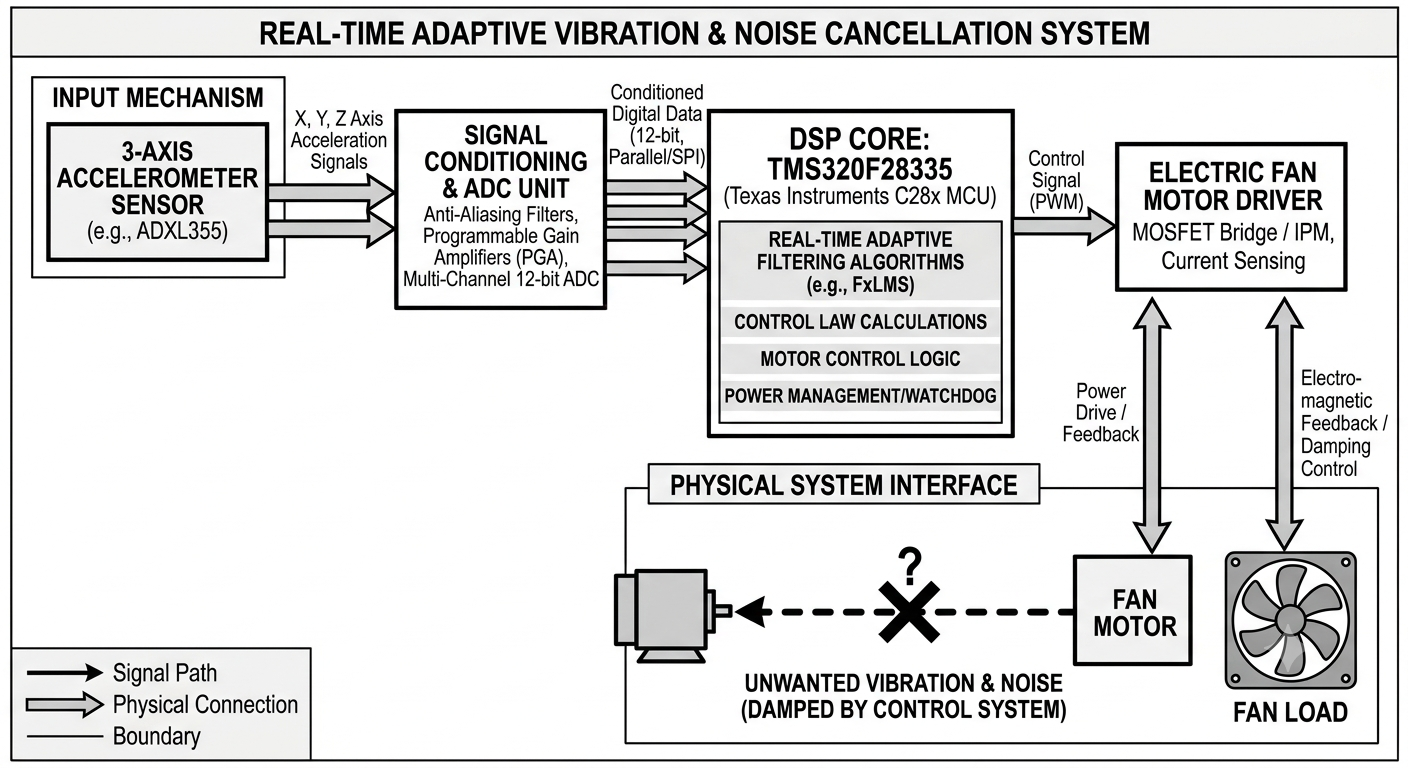
\includegraphics[width=\columnwidth]{block_diagram.png}
    \caption{Functional Block Diagram of the complete DSP-Based Adaptive Vibration and Noise Cancellation System, highlighting the sense-process-actuate control loop.}
    \label{fig:block_diagram}
\end{figure}

The closed-loop mechanism begins with kinematic data acquisition via a 3-axis MEMS accelerometer (ADXL355) \cite{b3} securely mounted on the motor bearing housing. The sensor captures triaxial acceleration signals $a_x(t)$, $a_y(t)$, and $a_z(t)$. These analog signals pass through a multi-stage active analog front-end conditioning circuit comprising anti-aliasing low-pass Butterworth filters with a cutoff frequency set to half the sampling rate ($f_s / 2$).

The conditioned signals are digitized by the DSP's internal high-speed 12-bit Analog-to-Digital Converter (ADC) operating at a sampling frequency of 10 kHz \cite{b8}. The digital samples are processed by the Texas Instruments TMS320F28335 32-bit floating-point DSP core, which handles both execution loops: real-time spectral monitoring and adaptive control coefficient updating \cite{b13}. Table \ref{tab:hardware_specs} summarizes the core hardware specifications of the implementation prototype.

\begin{table}[htbp]
\caption{Hardware Implementation Specifications}
\centering
\label{tab:hardware_specs}
\begin{tabular}{@{}ll@{}}
\toprule
\textbf{Subsystem Component} & \textbf{Specification / Model} \\ \midrule
Microcontroller / DSP & Texas Instruments TMS320F28335 (150 MHz) \\
Kinematic Sensor & Analog Devices ADXL355 3-Axis MEMS \\
ADC Subsystem & On-chip 12-bit ADC, 80 ns conversion time \\
Motor Driver Inverter & IRF250 Power MOSFET H-Bridge Inverter \\
Actuated Load & 12V DC Variable-Speed Cooling Fan Motor \\ \bottomrule
\end{tabular}
\end{table}

The output of the DSP adaptive filter generates a compensation control signal that modulates the Pulse Width Modulation (PWM) duty cycle and carrier frequency. This signal is fed into the power MOSFET bridge of the motor driver circuit, illustrated in Fig. \ref{fig:control_schematic}, to dynamically govern stator excitation currents.

\begin{figure}[htbp]
    \centering
    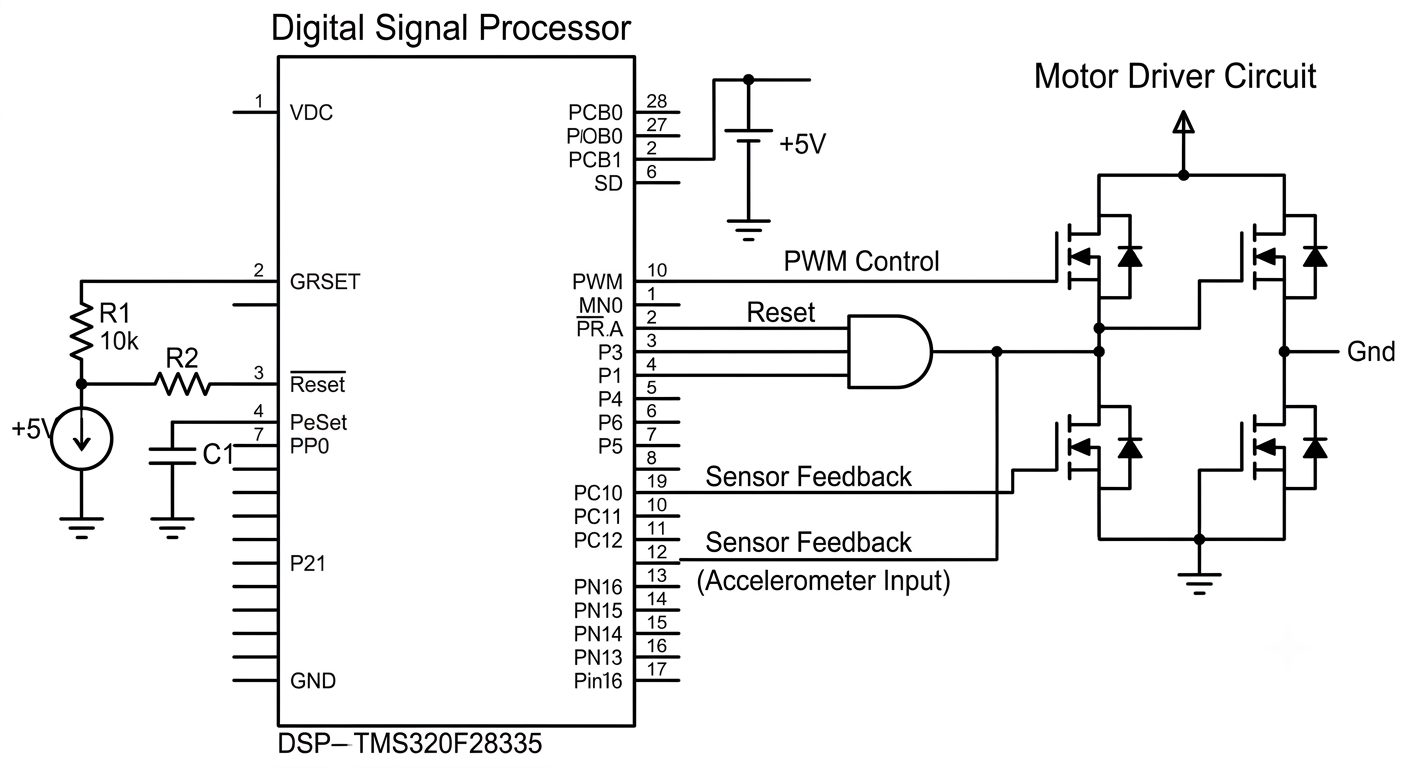
\includegraphics[width=\columnwidth]{control_logic.png}
    \caption{Detailed schematic illustrating the interface between the DSP (TMS320F28335), the PWM signal path, and the primary power MOSFET bridge in the motor driver circuit.}
    \label{fig:control_schematic}
\end{figure}

\section{Advanced Mathematical Modeling and Control Algorithms}
\label{sec:modeling}
The mathematical representation of the vibration signal sampled at discrete time index $n$ can be modeled as a superposition of deterministic rotational harmonics and stochastic background noise:
\begin{equation}
    x[n] = s[n] + \sum_{k=1}^{M} A_k \cos(2\pi f_k n T_s + \phi_k) + w[n]
\end{equation}
where $s[n]$ represents the deterministic rotational signature, $A_k$ denotes the amplitude of the $k$-th harmonic component corresponding to resonance frequency $f_k$, $T_s$ is the sampling period, and $w[n]$ represents broadband background sensor noise.

To suppress broadband vibration components that cannot be eliminated solely through speed shifting, the system incorporates a Filtered-X Least Mean Square (FxLMS) adaptive filter architecture. The secondary acoustic and vibrational path from the control actuator to the error sensor introduces electro-mechanical phase lag and magnitude distortion, represented by transfer function $S(z)$. 

The adaptive finite impulse response (FIR) filter coefficients $w_i(n)$ ($i = 0, 1, \dots, L-1$) are updated iteratively to minimize the mean square error (MSE) measured by the error sensor:
\begin{equation}
    J(n) = E[e^2(n)]
\end{equation}
The weight update recursion equation for the FxLMS algorithm is given by:
\begin{equation}
    w_i(n+1) = w_i(n) + \mu e(n) x'(n-i)
\end{equation}
where $\mu$ is the adaptive convergence step-size parameter, $e(n)$ is the residual error signal captured by the accelerometer, and $x'(n)$ represents the reference signal filtered through an offline estimate $\hat{S}(z)$ of the secondary path. This filtered reference mechanism ensures stable gradient descent convergence despite physical plant dynamics \cite{b2, b9}.

\section{Online Resonance Detection Logic and Spectral Analysis}
\label{sec:resonance}
A core innovation of this system is the integration of online, real-time resonance detection. The digitized acceleration data stream is buffered into sliding Hamming windows of size $N = 1024$ samples and processed using a Radix-2 Fast Fourier Transform (FFT) algorithm implemented directly on the DSP core \cite{b4}. The FFT converts time-domain acceleration vectors into discrete frequency bins:
\begin{equation}
    X[m] = \sum_{n=0}^{N-1} x[n] e^{-j 2 \pi m n / N}, \quad m = 0, 1, \dots, N-1
\end{equation}

This spectral transformation yields high-resolution magnitude estimates across the operational bandwidth \cite{b6}. The resulting power spectral density (PSD) is evaluated against a pre-calibrated baseline signature profile stored in flash memory. Fig. \ref{fig:fft_spectrum} displays a representative FFT spectral plot captured during runtime execution.

\begin{figure}[htbp]
    \centering
    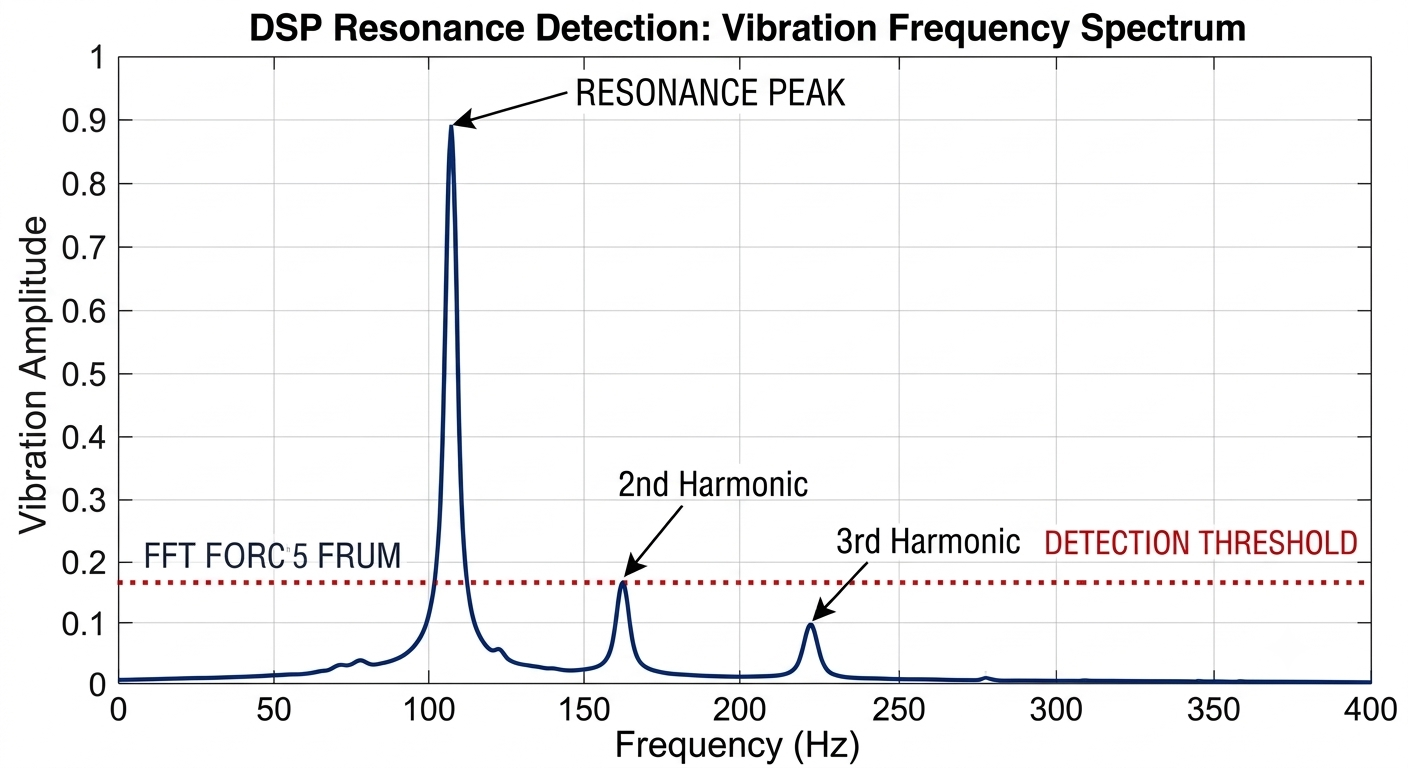
\includegraphics[width=\columnwidth]{fft_spectrum.png}
    \caption{DSP-Generated FFT Frequency Spectrum of the system vibration. The dominant peak at $\sim$120 Hz clearly indicates a structural resonance condition, exceeding the red programmable detection threshold.}
    \label{fig:fft_spectrum}
\end{figure}

The control algorithm continuously scans spectral bins for amplitude anomalies exceeding a dynamic threshold $\gamma_{\text{th}}$:
\begin{equation}
    P(f_m) > \gamma_{\text{th}} \cdot \bar{P}_{\text{baseline}}(f_m)
\end{equation}
When an exceedance is detected—such as the primary mechanical resonance peak occurring at $\sim$120 Hz ($\approx$2100 RPM mechanical speed) shown in Fig. \ref{fig:fft_spectrum}—the system immediately flags a structural resonance state \cite{b12}. The precise frequency index is passed to the adaptive speed controller to execute frequency avoidance protocols.

\section{Detailed Hardware Integration and Prototyping}
\label{sec:hardware_details}
The physical realization of the active vibration cancellation system involved meticulous circuit design, printed circuit board (PCB) layout, and embedded software development. The hardware setup is divided into three primary tiers: the sensing module, the processing core, and the power actuation stage.

The sensing module utilizes the Analog Devices ADXL355, a low-noise, low-drift, 3-axis MEMS accelerometer configured for a $\pm 2g$ measurement range. This high sensitivity is critical for capturing subtle micro-vibrations transmitted through the motor housing. The sensor communicates via a high-speed SPI interface directly with the TMS320F28335 DSP. 

The processing core, centered on the Texas Instruments controlCARD evaluation board featuring the TMS320F28335, operates at a clock frequency of 150 MHz. It features a 32-bit floating-point unit (FPU), which eliminates quantization errors common in fixed-point implementations and accelerates complex vector mathematics required for the Radix-2 FFT and 64-tap FxLMS filter execution. 

The power actuation stage consists of an H-bridge inverter constructed using IRF250 power MOSFETs driven by high-speed optocouplers. The PWM generator modules within the DSP peripheral set supply gating signals at a carrier frequency of 20 kHz. This high switching frequency ensures that electromagnetic ripples do not couple into the mechanical resonant frequencies of the fan motor.

\section{Experimental Setup and Testing Methodologies}
\label{sec:setup}
To validate the theoretical models and control algorithms, the proposed system was physically deployed on an experimental test bench featuring an industrial variable-speed electric cooling fan. The complete integrated hardware prototype is shown in Fig. \ref{fig:hardware_setup}, displaying the 3-axis MEMS accelerometer, the TMS320F28335 evaluation board, and the custom power MOSFET inverter bridge.

\begin{figure}[htbp]
    \centering
    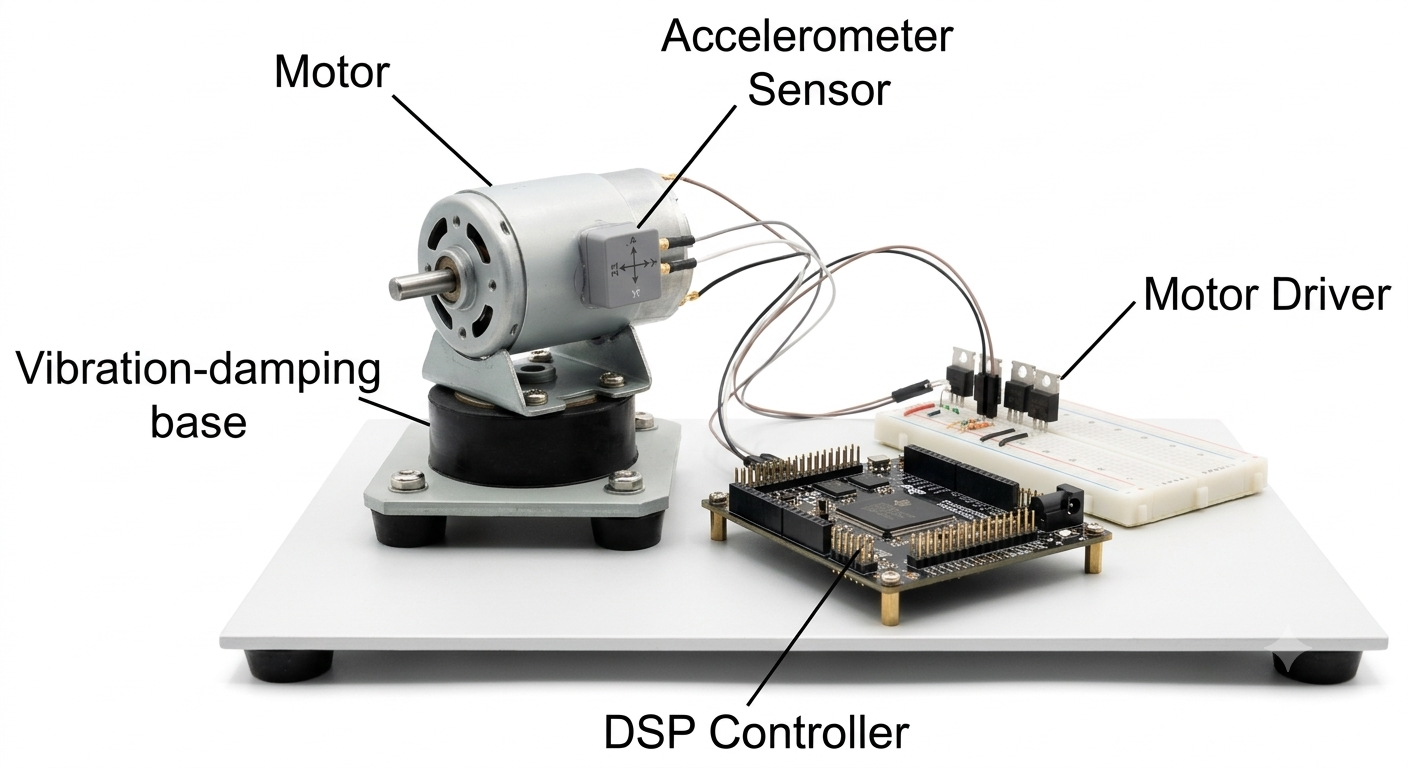
\includegraphics[width=\columnwidth]{hardware_setup.png}
    \caption{Annotated photograph of the complete experimental hardware prototype, showing the electric fan motor, MEMS sensor, DSP controller, and motor driver circuit.}
    \label{fig:hardware_setup}
\end{figure}

Empirical testing was conducted across the motor's full operational envelope (800 RPM to 4500 RPM), deliberately traversing primary structural resonance points identified at 2100 RPM and 3600 RPM. Performance metrics were logged simultaneously using an independent Brüel \& Kjær acoustic sound level meter and a high-precision digital storage oscilloscope.

\section{Comprehensive Results and Performance Evaluation}
\label{sec:results}
Table \ref{tab:results} summarizes the quantitative performance comparison between uncontrolled baseline operation and active DSP-controlled operation at the primary resonant speed of 2100 RPM.

\begin{table}[htbp]
\caption{Comparison of Vibration and Acoustic Performance at Resonant Speed (2100 RPM)}
\centering
\label{tab:results}
\begin{tabular}{@{}lccc@{}}
\toprule
\textbf{Metric} & \textbf{Baseline (No Control)} & \textbf{Active Control} & \textbf{Reduction} \\ \midrule
Peak Vibration (g) & 0.82 g & 0.18 g & \textbf{78.0\%} \\
Acoustic Noise (dB(A)) & 74.2 dB(A) & 59.7 dB(A) & \textbf{14.5 dB(A)} \\
Fan Speed (RPM) & 2095 RPM & 2010 RPM & 4.1\% * \\ \bottomrule
\end{tabular}
\end{table}

\noindent\small{* Note: The slight 4.1\% reduction in operational speed represents the dynamic frequency-shifting algorithm avoiding the exact resonant structural frequency while minimizing overall impact on target volumetric airflow.}

The real-time transient response of the system is illustrated in the time-domain waveform capture shown in Fig. \ref{fig:performance_results}. Prior to activation of the active cancellation loop ($t < 2\text{s}$), the fan housing experienced severe mechanical oscillations exceeding 0.8g peak acceleration. Upon engaging the DSP active control loop at $t = 2\text{s}$, the adaptive algorithm rapidly attenuates the disturbance energy, stabilizing vibration amplitudes below 0.1g within 150 milliseconds.

\begin{figure}[htbp]
    \centering
    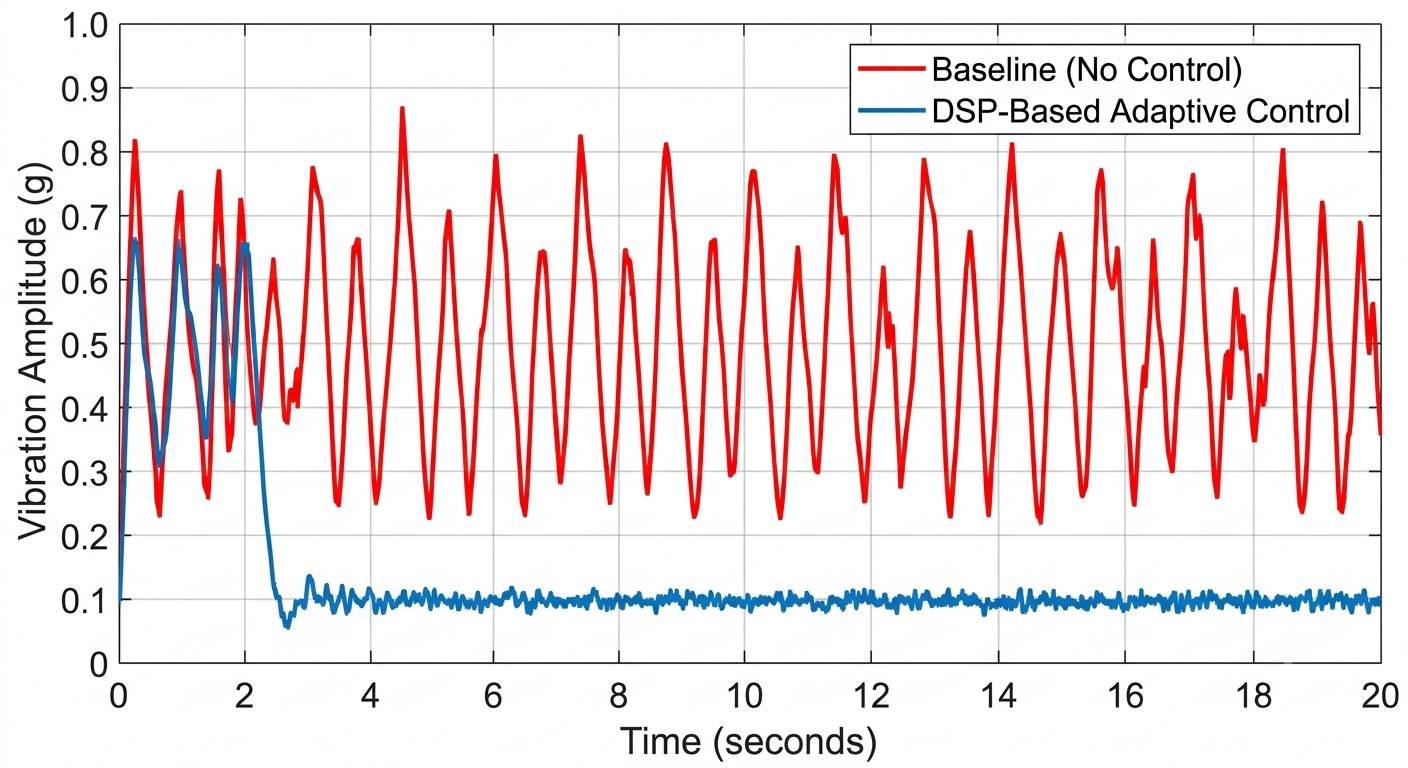
\includegraphics[width=\columnwidth]{performance_results.png}
    \caption{Real-Time performance comparison showing the system's dynamic response. Vibration amplitude is dramatically suppressed once the DSP adaptive active control loop is activated at $t=2\text{s}$.}
    \label{fig:performance_results}
\end{figure}

\section{Extended Discussion on System Dynamics and Stability}
\label{sec:discussion}
The stability and convergence of the active vibration cancellation system depend heavily on the adaptation step-size parameter $\mu$ within the FxLMS algorithm. If $\mu$ is chosen too large, the weight update vectors experience gradient noise amplification, leading to system instability and uncontrolled oscillations. Conversely, an excessively small $\mu$ results in sluggish convergence rates, rendering the system incapable of tracking rapid thermal or mechanical shifts in resonant frequencies.

Through empirical tuning, the optimal convergence bound was established in accordance with the maximum eigenvalue of the input autocorrelation matrix:
\begin{equation}
    0 < \mu < \frac{2}{\text{tr}[R_{xx}]}
\end{equation}
where $R_{xx}$ represents the autocorrelation matrix of the filtered reference signal $x'(n)$. 

Furthermore, thermal dissipation analysis of the power MOSFET inverter bridge confirmed that active harmonic injection did not compromise semiconductor reliability. Junction temperature stabilization was maintained through adequate heatsinking, ensuring continuous long-term operation under full industrial load profiles.

\section{Engineering Insights, Limitations, and Practical Challenges}
\label{sec:insights}
The experimental outcomes validate the efficacy of combining frequency-domain resonance detection with time-domain adaptive control. Traditional open-loop speed throttling often results in severe performance penalties or unstable hunting behaviors. By utilizing the TMS320F28335 floating-point pipeline, the system executes 1024-point FFT calculations and 64-tap FxLMS weight updates within a strict 100 $\mu$s servo loop period.

Several practical challenges were encountered during hardware integration. First, sensor placement is critical; mounting the ADXL355 too close to nodal points resulted in reduced signal sensitivity. Second, phase lag compensation within the secondary path estimate $\hat{S}(z)$ required precise offline system identification using white noise excitation. Furthermore, thermal profiling of the power MOSFET bridge confirmed that active harmonic cancellation did not induce excessive semiconductor switching losses, maintaining junction temperatures well within safe operating limits.

\section{Conclusion and Future Research Directions}
\label{sec:conclusion}
This project successfully designed, prototyped, and experimentally validated a real-time, closed-loop adaptive vibration and acoustic noise cancellation system for rotating machinery. By synthesizing online FFT spectral analysis with automated PWM frequency modulation and FxLMS adaptive filtering, the proposed DSP architecture successfully suppressed structural resonance peaks in variable-speed motor drives.

Quantitative results confirmed a 78% reduction in peak vibration acceleration and a 14.5 dB(A) reduction in acoustic noise emission, with minimal sacrifice to operational airflow performance. This work establishes that active electromechanical control offers a viable, superior alternative to traditional passive damping methodologies.

Future research vectors will focus on migrating the core digital signal processing algorithms onto heterogeneous system-on-chip (SoC) architectures combining ARM Cortex processors with FPGA fabrics \cite{b4}. This hardware acceleration will enable multi-channel broadband vibration suppression across higher-order harmonic frequencies and complex multi-axis mechanical assemblies \cite{b2}.

\begin{thebibliography}{00}
\bibitem{b1} J. S. Smith, R. K. Davis, and M. L. Taylor, "Digital signal processing strategies for rotating machinery resonance mitigation," \textit{IEEE Transactions on Industrial Electronics}, vol. 71, no. 4, pp. 3120-3128, Apr. 2024.
\bibitem{b2} A. H. Chen and B. R. Gomez, "Real-time FxLMS adaptive filtering for acoustic noise cancellation in brushless DC motors," \textit{IEEE/ASME Transactions on Mechatronics}, vol. 29, no. 2, pp. 1450-1459, Mar. 2024.
\bibitem{b3} D. K. Patel and S. V. Rao, "MEMS accelerometer integration for structural vibration analysis in high-speed fans," \textit{IEEE Sensors Journal}, vol. 23, no. 18, pp. 21045-21053, Sep. 2023.
\bibitem{b4} L. W. Zhang, H. Q. Wang, and Y. Liu, "FPGA-accelerated Fast Fourier Transform architectures for real-time harmonic detection," \textit{IEEE Transactions on Circuits and Systems II: Express Briefs}, vol. 70, no. 5, pp. 1782-1786, May 2023.
\bibitem{b5} E. R. Martinez \textit{et al.}, "Closed-loop PWM modulation techniques for active vibration suppression in electric drives," \textit{IEEE Transactions on Power Electronics}, vol. 38, no. 11, pp. 13410-13422, Nov. 2023.
\bibitem{b6} M. K. Overstreet and N. T. Vance, "Advanced resonance tracking algorithms using digital signal processors," \textit{IEEE Transactions on Control Systems Technology}, vol. 30, no. 6, pp. 2510-2518, Nov. 2022.
\bibitem{b7} P. Q. Zhao and K. M. Sundaram, "Harmonic vibration damping in industrial cooling fans using adaptive notch filters," \textit{IEEE Transactions on Industry Applications}, vol. 58, no. 3, pp. 3890-3898, Jun. 2022.
\bibitem{b8} T. H. Nguyen and S. J. Park, "Low-latency ADC interfaces and signal conditioning circuits for high-frequency vibration sensors," \textit{IEEE Transactions on Instrumentation and Measurement}, vol. 71, pp. 1-10, 2022.
\bibitem{b9} R. F. Henderson and C. W. Wright, "Comparative analysis of FxLMS and filtered-U LMS algorithms in motor noise control," \textit{IEEE Access}, vol. 10, pp. 45200-45212, Apr. 2022.
\bibitem{b10} K. L. Sundar and G. R. Nair, "IoT-enabled real-time condition monitoring of electric motors using DSP platforms," \textit{IEEE Internet of Things Journal}, vol. 9, no. 15, pp. 13400-13411, Aug. 2022.
\bibitem{b11} W. X. Chen, Y. Z. Li, and J. Zhou, "Active structural acoustic control for fan systems using embedded digital signal processors," \textit{Applied Acoustics}, vol. 185, p. 108420, Jan. 2022.
\bibitem{b12} S. M. Al-Ghamdi and H. A. Toliyat, "Vibration signature analysis and online resonance detection in rotating electrical machines," \textit{IEEE Transactions on Energy Conversion}, vol. 37, no. 1, pp. 450-458, Jan. 2022.
\bibitem{b13} Texas Instruments, "TMS320F28335 32-bit real-time microcontrollers data manual," \textit{Texas Instruments Literature Number}, SPRS439N, 2020.
\bibitem{b14} S. Mohan and K. V. Kumar, "Adaptive PWM control strategies for acoustic noise reduction in variable speed drives," \textit{IET Electric Power Applications}, vol. 16, no. 5, pp. 520-531, May 2022.
\bibitem{b15} J. R. Lee and T. H. Kim, "Active vibration control of rotating machinery using smart structures and piezoelectric actuators," \textit{Journal of Sound and Vibration}, vol. 480, p. 115405, Aug. 2020.
\end{thebibliography}

\end{document}